%%%%%%%%%%%%%%%%%%%%%%%%%%%%%%%%%%%%%%%%%%%%%%%%%%%%%%%%%%%%
%%% arXiv preprint — style vendored locally (arxiv.sty).
%%% Build with pdflatex (latexmk -pdf); see README.
%%%%%%%%%%%%%%%%%%%%%%%%%%%%%%%%%%%%%%%%%%%%%%%%%%%%%%%%%%%%
\documentclass{article}

\usepackage{arxiv}

\usepackage[utf8]{inputenc}
\usepackage[T1]{fontenc}
\usepackage{graphicx}
\graphicspath{{figures/}}
\usepackage{amsmath}
\usepackage{amssymb}
\usepackage[numbers]{natbib}
\usepackage{hyperref}
% Let bare underscores print in text mode (DOIs in the bibliography contain
% them); leaves math-mode subscripts untouched.
\usepackage{underscore}

\renewcommand{\headeright}{Preprint}
\renewcommand{\undertitle}{Preprint}

%%%%%%%%%%%%%%%%%%%%%%%%%%%%%%%%%%%%%%%%%%%%%%%%%%%%%%%%%%%%
%%% Article setup
%%%%%%%%%%%%%%%%%%%%%%%%%%%%%%%%%%%%%%%%%%%%%%%%%%%%%%%%%%%%
\title{paper001}

\author{
  Eoin Murray \\
  Department of Engineering \\
  University of Cambridge \\
  \And
  Timothy O'Leary \\
  Department of Engineering \\
  University of Cambridge \\
}

\begin{document}
\maketitle

\begin{abstract}

Bullet points for now.

\end{abstract}

\section{Introduction}

Introduction is bullets for now, to be completed after methods and results.

Gamma in the brain, it oscillates in the 30-80 Hz band, and is implicated in attention, binding and gating \citep{buzsaki2012mechanisms, fries2015rhythms}, with the original empirical link being gamma in the visual cortex \citep{fries2001modulation}.

Gamma is thought to come from ING and PING, only PING will be investigated here (cite needed for ING).

PING is an emergent property of recurrent EI connections \citep{borgers2017ping, borgerskopell2003synchronization, borgerskopell2005effects}, backed by causal experimental evidence that fast-spiking interneurons generate the rhythm \citep[in vitro,][]{whittington1995synchronized} \citep[via optogenetics,][]{cardin2009driving, sohal2009parvalbumin}, and by the interneuron synaptic mechanisms that synchronise it \citep{bartos2007synaptic}.

We will discuss the state of the art in modelling PING \citep{kopell2010gamma, viriyopase2016cooperation}, and neural mass models and mean field models \citep{wilson1972excitatory, segneri2020theta, nandi2024bursting}. Note here all these model PING, non train it.

Introduction to spiking neural networks with surrogate gradient descent \citep{neftci2019surrogate, eshraghian2023training}. Note these trained networks are current based and non-rhythmic. Or when they are rhythmic the rhythm is injected rather than self organised \citep{yan2025efficient}.

We report a trained PING where the E rate is 10x lower than the non-PING counterpart, while this depends on an increase in the I spikes, it is still relevant because in the cortex I spikes are less costly than E spikes \citep{attwell2001energy, howarth2012updated}.

Biological pyramidal cells fire at low (less than 10Hz) rates, despite strong input \citep{barth2012experimental}. We propose that gamma holds down the rates.

The rate-vs-timing framing: classical views treat rate and spike timing as competitors; we show a regime where the rhythm sets the rate, so the two are one quantity \citep{ainsworth2012rates}.

This work: we train a PING network on a task for the first time, and show the architecture-generated gamma rhythm gates the excitatory population to an order-of-magnitude-lower spike rate at matched accuracy.

The headline claim in one line: gamma gating buys a per-spike economy that is supplied by the architecture, not learned — and it operates online, on continuous input streams, as cortical processing must.

Roadmap of the paper: build the model (Section~\ref{claim:1}), locate the onset in theory + data (Section~\ref{claim:2}), show the trained economy (Section~\ref{claim:3}), prove it is architectural not learned (Section~\ref{claim:4}), pin the rate to the clock (Section~\ref{claim:5}), test the dynamics for robustness (Section~\ref{claim:6}), and demonstrate streaming use (Section~\ref{claim:7}).

\section{Results}

\subsection{The model: COBA baseline and the PING loop}
\label{claim:1}

With the loop disengaged ($W_{ei} = W_{ie} = 0$) the network reduces to a COBA baseline that fires asynchronously, with no spectral gamma peak and an E $f$--$I$ curve that saturates near $270$~Hz under strong drive. Engaging the loop produces synchronous I bursts, gamma-banded E rasters with a clean PSD peak at $f_\gamma \approx 25$~Hz, and an E firing rate held roughly an order of magnitude below the COBA baseline across two decades of input drive (Figure~\ref{fig:1}). A single E$\to$I$\to$E loop thus generates the rhythm and clamps the E rate at the same time.

\subsection{\texorpdfstring{Gamma onset across the $W_{ei} \times W_{ie}$ plane}{Gamma onset across the W_ei x W_ie plane}}
\label{claim:2}

Across the $W_{ei} \times W_{ie}$ coupling plane the E rate falls, the I rate rises, and the lobe--trough rhythmicity score $R$ grows together --- $R \approx 0$ along the two COBA edges and rising smoothly to $R \approx 0.9$ toward strong coupling. The 4D mean-field reduction of \emph{Methods} predicts a supercritical Hopf at external drive $I_\mathrm{ext}^\star = 0.59$~nA and crossing frequency $f^\star \approx 24.5$~Hz, confirmed by reversible quasi-static up/down ramps with vanishing hysteresis and $A^2 \propto (I_\mathrm{ext} - I_\mathrm{ext}^\star)$ at $R^2 = 0.999$; the predicted gamma frequency tracks the spiking measurement across $\tau_\mathrm{GABA} \in [4.5, 27]$~ms (Figure~\ref{fig:2}). The smooth empirical onset is what a supercritical Hopf predicts.

\subsection{\texorpdfstring{Trained PING matches COBA accuracy at $\approx 10\times$ fewer spikes}{Trained PING matches COBA accuracy at approximately 10x fewer spikes}}
\label{claim:3}

Trained on MNIST with surrogate-gradient descent (\emph{Training}), both architectures converge to $\approx 83\%$ test accuracy. Sweeping the spike-budget penalty $\theta_u$ traces an accuracy--rate frontier on which PING sits up-and-left of COBA at every point: at the $\theta_u$-off operating point PING reaches $\approx 83\%$ at a mean hidden-E rate of $\approx 3.8$~Hz, against COBA's $\approx 90\%$ at $\approx 56$~Hz (Figure~\ref{fig:3}). The rate floor is structural and the trained PING locks to it as a stable attractor: it cannot be trained away by lowering $\theta_u$, and the trained rate is robust across seeds.

\subsection{Sparsity is supplied by the architecture, not learned}
\label{claim:4}

Switching the recurrent loop on \emph{at inference} on a trained COBA, with no retraining of any weight, immediately produces gamma bands in the raster and drops the mean E rate by $\approx 10\times$ ($\approx 60 \to 5$~Hz); accuracy without retraining degrades by $\approx 24$~pp (Figure~\ref{fig:4}). The converse test --- unfreezing the loop weights $W_{ei}$, $W_{ie}$ and letting Adam train them under the Dale's-law clamp --- has gradient descent \emph{prune} the loop away from every initialisation (PING, zero, small-seed): the I rate collapses to $\approx 0$~Hz within a few epochs, $R$ drains to $\sim 0.04$--$0.18$, and accuracy is unchanged (Figure~\ref{fig:5}). The architecture supplies the gating; training neither needs it nor finds it.

\subsection{The gamma clock sets the excitatory firing rate}
\label{claim:5}

Retraining the network at each $\tau_\mathrm{GABA}$ to vary $f_\gamma$ yields a post-training E rate that is affine in the gamma frequency, $r_E = 0.76 + 0.216 \, f_\gamma$ with $R^2 = 0.997$ across three seeds per point, and accuracy holds at $81$--$89\%$ throughout (Figure~\ref{fig:6}). The microscopic cause is direct: $99.45\%$ of (cell, cycle) pairs emit at most one spike, with $P(0) \approx 77\%$, $P(1) \approx 22\%$, and the multi-spike fraction below $\sim 3\%$ across the whole $\tau_\mathrm{GABA}$ sweep --- a cell either skips the cycle or contributes a single spike, with the I volley resetting the population in between (Figure~\ref{fig:7}). The rate knob is the per-synapse weight $W^{IE}$, not the I-pool headcount: sweeping $W^{IE}$ across $N_I \in \{16, 64, 256\}$ collapses all three E-rate curves onto a single line, so the loop scales by synaptic gain rather than by interneuron count (Figure~\ref{fig:8}).

\subsection{Dynamics and robustness of the gating}
\label{claim:6}

The gating lives in the \emph{timing} of inhibition, not its average. PING holds $\approx 82\%$ accuracy through an $80\%$ drop of emitted spikes --- silence is informative --- but falls off a cliff by $\approx 15\%$ relative added Poisson noise, because off-phase spikes drive the I pool at arbitrary phase and dissolve the rhythm; COBA, having no rhythm to protect, is the mirror image (Figure~\ref{fig:9}). Two inference-time jitter perturbations of the trained I stream that hold the mean per-cell I rate fixed drive the E rate in \emph{opposite} directions: per-I-cell jitter smears the bursts into a continuous shunt and the E rate collapses to zero, while cycle-coherent jitter preserves within-burst synchrony and the E rate rises from $\approx 8$~Hz toward $\approx 50$~Hz (Figure~\ref{fig:10}). The rate gap is the phase structure of inhibition, not its level. The result is a physical-Hz property: across a $20\times$ span of integration timestep ($\Delta t = 0.05 \to 1.0$~ms) the post-training E rate stays within an $8.4$--$12$~Hz band and accuracy is flat within $2.7$~pp (Figure~\ref{fig:11}).

\subsection{Streaming classification on continuous input}
\label{claim:7}

A PING trained on single MNIST digits classifies a continuously concatenated input stream with no retraining and no segmentation cue: re-identification of each new digit takes $\approx 1$ gamma cycle. The streaming protocol of \emph{Datasets and evaluation} --- the time-averaged readout of the non-spiking LIF output, applied to a sliding window matched to each segment's duration --- recovers $5/5$ correct on a representative stream where each digit is presented with its own duration ($25$--$200$~ms) and input rate ($10$--$200$~Hz) (Figure~\ref{fig:12}). On the full ($\tau$, input-rate) grid, accuracy is approximately a function of the product $\tau \cdot \mathrm{rate}$, with a hard sub-cycle failure floor below $\tau \approx 15$~ms: even at $200$~Hz the network cannot classify in less than one gamma cycle, identifying the cycle as the temporal quantum of the computation (Figure~\ref{fig:13}). The trained operating point ($200$~ms, $25$~Hz) sits at $88\%$, interior to a broad plateau.

\section{Discussion}
To be drafted.

\section{Methods}

\subsection{Single-neuron and synapse dynamics}

We use a conductance-based leaky integrate-and-fire (LIF) model with two populations, excitatory (E) and inhibitory (I). The sub-threshold membrane potential of each population evolves as

\begin{align}
  C_m^E \, \frac{dV^E}{dt} &= -g_L^E (V^E - E_L) - g_e^E (V^E - E_e) - g_i^E (V^E - E_i) \\
  C_m^I \, \frac{dV^I}{dt} &= -g_L^I (V^I - E_L) - g_e^I (V^I - E_e)
\end{align}

where $C_m$ is the membrane capacitance, $g_L$ the leak conductance, $E_L$ the leak reversal potential, and $E_e$, $E_i$ the excitatory and inhibitory synaptic reversal potentials. The I population has no inhibitory term because there is no I$\to$I connection in this architecture (\emph{Network architecture}, below).

A neuron emits a spike when $V$ crosses threshold $V_\mathrm{th}$ from below; its potential is then clamped to $V_\mathrm{reset}$ for a refractory period $\tau_\mathrm{ref}$:

\begin{equation}
  s_{t+1} = \mathbf{1}\!\left[V \geq V_\mathrm{th}\right], \qquad V \leftarrow V_\mathrm{reset} \ \text{if } s_{t+1} = 1 \text{ or refractory}.
\end{equation}

Each synaptic conductance is an exponential trace driven by presynaptic spikes: a presynaptic spike adds its full weight $W$ as an instantaneous jump in conductance, which then decays with the relevant channel time constant ($\tau_\mathrm{AMPA}$ for AMPA-like excitation, $\tau_\mathrm{GABA}$ for GABA-like inhibition):

\begin{align}
  \frac{dg^E_e}{dt} &= -\frac{g^E_e}{\tau_\mathrm{AMPA}} + W_\mathrm{in} \sum_k \delta(t - t^\mathrm{inp}_k) \label{eq:gE_e} \\
  \frac{dg^E_i}{dt} &= -\frac{g^E_i}{\tau_\mathrm{GABA}} + W_{ie}      \sum_k \delta(t - t^{i}_k)        \label{eq:gE_i} \\
  \frac{dg^I_e}{dt} &= -\frac{g^I_e}{\tau_\mathrm{AMPA}} + W_{ei}      \sum_k \delta(t - t^{e}_k)        \label{eq:gI_e}
\end{align}

Equation~\eqref{eq:gE_e} is the input-driven excitation onto E via feedforward weights $W_\mathrm{in}$; \eqref{eq:gE_i} is the inhibition onto E from I via $W_{ie}$; \eqref{eq:gI_e} is the excitation onto I from E via $W_{ei}$. There is no equation for $g^I_i$ (no I$\to$I connection) and no recurrent contribution to $g^E_e$ (no E$\to$E connection); see \emph{Network architecture}. Canonical values are listed in Table~\ref{tab:params}; E and I populations differ in membrane capacitance, leak conductance, membrane time constant, and refractory period.

\begin{table}[!htbp]
\centering
\caption{Canonical (``default'') parameter values for the spiking neural network. Where E and I populations use different values they are listed as ``E~/~I''; otherwise the value is shared. The $\tau_\mathrm{GABA} = 9$~ms value matches the canonical PING choice in \citet{borgers2017ping}.}
\label{tab:params}
\begin{tabular}{lll}
\hline
Symbol & Description & Value \\
\hline
$C_m$                & Membrane capacitance         & $1.0$ / $0.5$~nF \\
$g_L$                & Leak conductance             & $0.05$ / $0.1$~$\mu$S \\
$\tau_m$             & Membrane time constant       & $20$ / $5$~ms \\
$\tau_\mathrm{ref}$  & Refractory period            & $3.0$ / $1.5$~ms \\
$E_L$                & Leak reversal potential      & $-65$~mV \\
$V_\mathrm{th}$      & Spike threshold              & $-50$~mV \\
$V_\mathrm{reset}$   & Reset potential              & $-65$~mV \\
$E_e$                & AMPA reversal potential      & $0$~mV \\
$E_i$                & GABA reversal potential      & $-80$~mV \\
$\tau_\mathrm{AMPA}$ & AMPA decay time constant     & $2$~ms \\
$\tau_\mathrm{GABA}$ & GABA decay time constant     & $9$~ms \\
$\Delta t$           & Integration timestep         & $0.1$~ms (train) / $0.25$~ms (inference) \\
$N_E$                & Hidden excitatory pool size  & $1024$ \\
$N_I$                & Inhibitory pool size         & $256$ \\
\hline
\end{tabular}
\end{table}

\subsection{Network architecture}

The network has one hidden layer with $N_E$ excitatory and $N_I$ inhibitory units; a non-spiking leaky-integrator readout layer with weights $W_\mathrm{out}$ over the E population produces classification logits. The readout units follow LIF membrane dynamics with no spike, reset, or refractory period; the per-class logits are their membrane potentials averaged over the presentation window. Input spikes drive E via feedforward weights $W_\mathrm{in}$. Recurrence is restricted to the E$\leftrightarrow$I loop: E projects to I via $W_{ei}$, I projects back to E via $W_{ie}$. There is no $W_{ee}$ and no $W_{ii}$.

This minimal recurrence is deliberate. PING and ING are the two well-characterised gamma-generation mechanisms in cortex; by excluding $W_{ii}$ we rule out ING, and by excluding $W_{ee}$ we rule out recurrent-E driven oscillation, so any rhythm that emerges is unambiguously PING (E$\leftrightarrow$I) \citep{borgers2017ping, viriyopase2016cooperation}. The conductance-based (COBA) baseline used as a non-PING control throughout the paper is the loop-off limit of the same architecture, obtained by setting $W_{ei} = W_{ie} = 0$.

The loop weights $W_{ei}$ and $W_{ie}$ are fixed (untrained) throughout this work. We treat the loop as a structural prior, not as a feature to be learned. This matches a functional distinction long made in the inhibitory-plasticity literature: inhibitory synapses serve an experience-dependent E/I balance role rather than carrying the feedforward computational features that the excitatory pathway learns \citep{vogels2011inhibitory, hennequin2017inhibitory}. The fixed-loop choice is also defended empirically by the result that allowing the loop to train causes gradient descent on MNIST to prune it away (Section~\ref{claim:4}, Figures~\ref{fig:4}--\ref{fig:5}). A Dale's-law clamp keeps the signs of all trained weights fixed throughout training (\emph{Training}, below).

\subsection{Mean-field reduction}

To locate the gamma-onset bifurcation analytically (Section~\ref{claim:2}) we reduce the spiking network to a deterministic four-dimensional rate model in the state
\begin{equation}
  \mathbf{x}(t) \;=\; \bigl(\bar{E},\; \bar{I},\; \bar{g}_e^I,\; \bar{g}_i^E\bigr),
\end{equation}
where $\bar{E}$ and $\bar{I}$ are the population-mean firing rates of the E and I cells (in spikes per millisecond), and $\bar{g}_e^I$, $\bar{g}_i^E$ are the population-mean cross-population synaptic conductances onto the I and E populations respectively. The two cross-population conductances are sufficient because the architecture has no $W_{ee}$ and no $W_{ii}$ (see \emph{Network architecture}); the within-population conductances vanish identically.

\paragraph{Population-mean equations.} The reduction replaces the spike-driven conductance dynamics of \eqref{eq:gE_e}--\eqref{eq:gI_e} with rate-driven first-order filters, and replaces each cell's stochastic spike output with the population-averaged firing rate of a noise-driven LIF cell at a given mean input current. The closed 4D system is
\begin{align}
  \tau_E \, \dot{\bar{E}}                    &= -\bar{E}      + \Phi_E\!\bigl(I_\mathrm{ext} - \bar{g}_i^E \, \Delta V_\mathrm{inh}\bigr) \label{eq:mf_E} \\
  \tau_I \, \dot{\bar{I}}                    &= -\bar{I}      + \Phi_I\!\bigl(\bar{g}_e^I \, \Delta V_\mathrm{exc}\bigr) \\
  \tau_\mathrm{AMPA} \, \dot{\bar{g}}{}_e^I &= -\bar{g}_e^I + \tau_\mathrm{AMPA} \, W^{EI} \, \bar{E} \\
  \tau_\mathrm{GABA} \, \dot{\bar{g}}{}_i^E &= -\bar{g}_i^E + \tau_\mathrm{GABA} \, W^{IE} \, \bar{I} \label{eq:mf_giE}
\end{align}
with $I_\mathrm{ext}$ an external tonic drive to E (the bifurcation control parameter, below), and driving forces $\Delta V_\mathrm{exc} = E_e - E_L = 65$~mV and $\Delta V_\mathrm{inh} = E_L - E_i = 15$~mV evaluated at rest. The membrane time constants $\tau_E$, $\tau_I$ and synaptic time constants $\tau_\mathrm{AMPA}$, $\tau_\mathrm{GABA}$ are taken directly from Table~\ref{tab:params}; the fan-in-normalised coupling strengths $W^{EI} = 1.0$~$\mu$S and $W^{IE} = 2.0$~$\mu$S are inherited from the same connectivity that is used in the spiking network.

\paragraph{Transfer function.} The population gain functions $\Phi_E$, $\Phi_I$ are the standard noise-driven LIF rate functions in Ricciardi--Siegert form. For mean input current $\mu$ delivered to a cell with leak conductance $g_L$, leak reversal $E_L$, threshold $V_\mathrm{th}$, reset $V_\mathrm{reset}$, membrane time constant $\tau_m$, and refractory period $\tau_\mathrm{ref}$,
\begin{equation}
  \Phi(\mu) \;=\; \left[\, \tau_\mathrm{ref} \;+\; \tau_m \sqrt{\pi} \int_{(V_\mathrm{reset} - \mu_V) / \sigma_V}^{(V_\mathrm{th} - \mu_V) / \sigma_V} e^{u^2} \bigl(1 + \mathrm{erf}\, u\bigr) \, du \,\right]^{-1},
  \label{eq:ricciardi}
\end{equation}
with mean membrane potential $\mu_V = E_L + \mu / g_L$ and effective membrane-noise scale $\sigma_V$; the integral is evaluated by numerical quadrature. All quantities entering $\Phi$ are taken from Table~\ref{tab:params}, separately for the E and I parameter sets. The only parameter not directly inherited from the spiking biophysics is the noise scale $\sigma_V$, set to $4$~mV; the Hopf location moves by less than $1$~Hz across $\sigma_V \in [3, 6]$~mV, so the bifurcation result is insensitive to this choice.

\paragraph{Bifurcation analysis.} We track the silent (non-oscillating) fixed point of \eqref{eq:mf_E}--\eqref{eq:mf_giE} as $I_\mathrm{ext}$ is swept from $0$ to $4$~nA in $10~\mu$A steps. At each value of $I_\mathrm{ext}$, the fixed point is obtained by solving the algebraic system in $(\bar{E}, \bar{I})$ --- at steady state the two conductances are slaved to the rates, $\bar{g}_e^I = \tau_\mathrm{AMPA} W^{EI} \bar{E}$ and $\bar{g}_i^E = \tau_\mathrm{GABA} W^{IE} \bar{I}$ --- using \texttt{scipy.optimize.fsolve}. The numerical Jacobian of the full 4D system at each fixed point is computed by central finite differences. The Hopf threshold $I_\mathrm{ext}^\star$ is the smallest $I_\mathrm{ext}$ at which the eigenvalue $\lambda^\star$ with largest real part crosses zero with non-zero imaginary part; the crossing frequency is $f^\star = |\mathrm{Im}\,\lambda^\star| / (2\pi)$.

\paragraph{Supercritical vs.\ subcritical classification.} We classify the onset numerically via a quasi-static amplitude sweep. $I_\mathrm{ext}$ is ramped up across $I_\mathrm{ext}^\star$ from a small perturbation of the silent fixed point, then ramped back down, integrating the 4D system to its steady-state oscillation amplitude $A$ at each step. The onset is classified as supercritical when (i) the up- and down-ramp branches coincide --- peak hysteresis gap below $10^{-4}$ in rate units --- and (ii) the squared amplitude scales linearly with the bifurcation distance above onset,
\begin{equation}
  A^2 \;\propto\; \bigl(I_\mathrm{ext} - I_\mathrm{ext}^\star\bigr),
\end{equation}
the Stuart--Landau normal-form signature, with $R^2 > 0.9$. For the canonical parameter set this criterion is met with hysteresis below $10^{-5}$ and $R^2 = 0.999$, confirming supercritical onset.

\paragraph{Comparison with the spiking network.} The mean-field prediction is compared against the gamma frequency measured in the full spiking network, extracted as in \emph{Measurement and analysis}, across a sweep of $\tau_\mathrm{GABA} \in \{4.5, 6, 9, 12, 18, 27\}$~ms (Figure~\ref{fig:2}). The two curves agree qualitatively --- both fall monotonically with $\tau_\mathrm{GABA}$ --- with a quantitative offset: the spiking network's synchronised E-volley dynamics produce a higher gamma frequency than the rate-equation prediction at every $\tau_\mathrm{GABA}$ in the swept range. The reduction nonetheless captures the dependence on the GABA decay time, which is what we use it for. This treatment follows the Wilson--Cowan and next-generation neural-mass tradition for cortical-rhythm modelling \citep{wilson1972excitatory, segneri2020theta}.

\subsection{Training}

Networks are trained on MNIST by surrogate-gradient descent through backpropagation in time \citep{neftci2019surrogate, eshraghian2023training}. Each digit is rate-encoded as a Poisson spike train over a 200~ms presentation window at a peak rate of 25~Hz per active pixel (Bernoulli per timestep with $p = r_\mathrm{max} \, \Delta t$). The loss is cross-entropy on the time-averaged membrane potentials of the non-spiking LIF readout, augmented by a per-neuron firing-rate penalty that activates only when a unit's mean rate exceeds a soft ceiling $\theta_u$:
\begin{equation}
  \mathcal{L} \;=\; \mathcal{L}_\mathrm{CE} \;+\; s_u \sum_{i \in E} \mathrm{ReLU}\!\left(\langle r_i \rangle - \theta_u\right)^2,
\end{equation}
where $\langle r_i \rangle$ is the per-trial mean spike count of E neuron $i$, $\theta_u$ is a per-neuron rate ceiling expressed in spikes per trial, and $s_u = 10^{-3}$ is the penalty strength. Sweeping $\theta_u$ over $\{\text{off}, 5, 2, 1, 0.5, 0.2\}$ spikes per 200~ms trial (equivalent peak rates of $25$, $10$, $5$, $2.5$, $1$~Hz) traces out the accuracy--rate frontier reported in Section~\ref{claim:3}.

The discrete spike nonlinearity has zero gradient almost everywhere; in the backward pass it is replaced by a fast-sigmoid surrogate of the distance to threshold $u = V - V_\mathrm{th}$,
\begin{equation}
  \frac{\partial \mathbf{1}[V \geq V_\mathrm{th}]}{\partial V} \;\equiv\; \frac{s}{(1 + s \, |u|)^2},
\end{equation}
with slope $s = 1$ \citep{neftci2019surrogate}; the forward pass evaluates the Heaviside exactly. Optimisation uses Adam with learning rate $4 \times 10^{-4}$, batch size $256$, and 100 epochs. Each baseline condition is repeated across three seeds ($42, 43, 44$); the spike-budget sweep uses a single seed (42).

\paragraph{Gradient damping for the PING case.} Surrogate-gradient training of the PING configuration is unstable without an additional intervention on the gradient. The closed E$\leftrightarrow$I recurrence means that a single loop weight ($W_{ei}$ or $W_{ie}$) contributes to the membrane-voltage update of every cell on every subsequent timestep within the trial; combined with the spike-driven impulse updates of the synaptic conductances in \eqref{eq:gE_e}--\eqref{eq:gI_e} and the surrogate's non-zero gradient at the spike threshold, this routes the gradient contribution through a tightly coupled feedback loop with millisecond-scale conductance dynamics. Over the $2{,}000$-step backpropagation-through-time window of a single $200$~ms MNIST trial at training step $\Delta t = 0.1$~ms, the contribution compounds multiplicatively across steps: gradient norms grow by many orders of magnitude through the recurrence and training does not converge. This is the spike-network analogue of the classical exploding-gradient pathology of recurrent networks, here driven by the conductance-based E$\leftrightarrow$I loop rather than by a saturating activation.

We address this by attenuating the gradient flowing through the membrane-voltage increment $dV$ on the backward pass by a factor of $1/d$, implemented as a straight-through identity that scales gradients without touching the forward value:
\begin{equation}
  \mathrm{damp}_d(x) \;=\; \tfrac{1}{d} \, x \;+\; \left(1 - \tfrac{1}{d}\right) \, \mathrm{stopgrad}(x).
\end{equation}
The operator is applied to $dV$ on every integration step of every layer, so the forward simulation is exact (the network still solves the same ODE) while the gradient flowing through that update is attenuated by a factor of $1/d$ per step, breaking the multiplicative compounding. We use $d = 1000$ for all paper figures, applied identically to the PING and the COBA-baseline pipelines so that the only training-pipeline difference between the two is the presence or absence of the recurrent loop weights. The COBA baseline (no loop) trains stably with the module-level default ($d = 80$); the PING configuration does not.

\paragraph{Dale's-law clamp.} After each optimiser step, weights are projected back to their sign cones: $W_\mathrm{in}$ and $W_{ei}$ are clipped to be non-negative, $W_{ie}$ to be non-positive. No synapse can change sign during training. This is what makes the loop-pruning result of Section~\ref{claim:4} meaningful: gradient descent is structurally allowed to strengthen the loop, and it does not.

\subsection{Measurement and analysis}

Mean firing rates $\langle r_E \rangle$ and $\langle r_I \rangle$ are computed as time-averaged spike counts per neuron over the presentation window. The gamma frequency $f_\gamma$ is extracted as the peak of the Welch power spectral density of the summed population E spike train at sampling rate $f_s = 1 / \Delta t = 4{,}000$~Hz, using a single segment of length equal to the trial, mean-centred (not z-scored) signal, no detrending, and a peak search restricted to the gamma band $[5, 150]$~Hz; the peak frequency is refined by parabolic sub-bin interpolation.

The rhythmicity score $R$ is the Michelson contrast between the first side lobe and the first trough of the autocorrelation of the binned population E spike count, computed via zero-padded FFT and normalised by the squared mean of the rate. After a 3-point smoothing kernel $[0.25, 0.5, 0.25]$ is applied to the autocorrelogram, the first trough is identified as the first local minimum starting from lag~2, and the lobe as the maximum between lag~1 and the trough; then
\begin{equation}
  R \;=\; \frac{\mathrm{lobe} - \mathrm{trough}}{\mathrm{lobe} + \mathrm{trough}} \;\in\; [0, 1).
\end{equation}
$R$ is bounded and scale-free, and was chosen because spectral-peak measures become noisy at low firing rates, where several of the regimes of interest in this paper sit; $R$ is qualitatively consistent with the spectral-peak and population-coherence measures used elsewhere in the gamma literature \citep{atallah2009instantaneous, xing2012stochastic}.

The spikes-per-cycle distribution (Figure~\ref{fig:7}) is built by binning each cell's spikes into the gamma cycles inferred from peaks of the population I-burst rate (Gaussian-smoothed with $\sigma = 1$~ms), detected with SciPy's \texttt{find\_peaks} requiring a minimum inter-peak separation of half the expected gamma period and a height $\geq 5\%$ of the maximum. Cycle boundaries are placed at midpoints between consecutive I-burst peaks; each E spike is assigned to its enclosing cycle.

Spike-economy claims report both the mean E rate and the total population spike count $N_E \langle r_E \rangle + N_I \langle r_I \rangle$, so the per-spike economy is stated net of the inhibitory pool. Excitatory spikes dominate cortical energy budgets \citep{attwell2001energy, howarth2012updated}; we do not build a network-specific metabolic model, and the economy claim is made in spike-count terms only.

\subsection{Integration and parameters}

The membrane and synaptic-conductance ODEs are integrated by an exponential-Euler scheme with zero-order hold on the synaptic conductances over each step. With $g_\mathrm{tot} = g_L + g_e + g_i$ the total instantaneous conductance, effective time constant $\tau_\mathrm{eff} = C_m / g_\mathrm{tot}$, and instantaneous steady state $V_\infty = (g_L E_L + g_e E_e + g_i E_i) / g_\mathrm{tot}$, the closed-form update is
\begin{equation}
  V_{t+1} \;=\; V_\infty \;+\; (V_t - V_\infty) \, e^{-\Delta t / \tau_\mathrm{eff}}.
  \label{eq:expeuler}
\end{equation}
We use $\Delta t = 0.1$~ms for training (finer steps are needed for stable backpropagation through the stiff E$\leftrightarrow$I recurrence) and the module-level default $\Delta t = 0.25$~ms for the trained-model inference runs that produce the paper figures. All rates and frequencies are reported in physical units (Hz), not per-step; the $\Delta t$-invariance check (Section~\ref{claim:6}, Figure~\ref{fig:11}) confirms that the reported quantities are well-defined as $\Delta t \to 0$ within the range used here.

The canonical operating point used by every ``default'' run --- pool sizes $N_E$, $N_I$; time constants $\tau_m$, $\tau_\mathrm{AMPA}$, $\tau_\mathrm{GABA}$, $\tau_\mathrm{ref}$; reversal potentials $E_L$, $E_e$, $E_i$; threshold and reset; and integration timestep --- is listed in Table~\ref{tab:params}. The loop weights $W_{ei}$, $W_{ie}$ and the input rate are stated per-experiment in the relevant figure caption, as are swept ranges (e.g.\ $\tau_\mathrm{GABA}$, $W_{ie}$).

\subsection{Datasets and evaluation}

The classification task is MNIST, rate-encoded as described in \emph{Training} (200~ms presentation, 25~Hz peak Poisson rate per active pixel). MNIST is used under its standard train/test split and we report test-set accuracy. For the streaming protocol used in Section~\ref{claim:7}, the trained network is presented with a continuously concatenated input stream and the argmax of the non-spiking LIF readout's membrane potentials is read out at each timestep as the streaming class label; the readout's own membrane time constant sets the integration window over which evidence is accumulated. Reported metrics are test accuracy, mean E and I firing rates, and $f_\gamma$.

\subsection{Reproducibility}

Each result has a standalone notebook script in the project repository (linked under \emph{Code and data availability}). Notebook runs use one of a small set of named size tiers (tiny, small, medium, large, huge), each with a fixed seed set and a per-tier compute budget; the tier and seed range used for each reported figure are recorded in the notebook header. The figure-render pipeline regenerates every print-quality figure from those notebooks, so a clean re-run of the repository reproduces the manuscript figures.

\subsection{Software and implementation}

The model, training, and analysis are implemented in Python ($\geq 3.10$). Spiking dynamics and surrogate-gradient training use PyTorch (2.11; with snnTorch 0.9 for baseline spiking primitives); numerical analysis uses NumPy (2.2) and SciPy (1.15); all figures are produced with Matplotlib (3.10).

\subsection{Generative-AI use}

Claude Code (Anthropic; model Opus 4.8), an agentic large-language-model coding tool, was used extensively and interactively throughout the development of this work. Its use covers: writing essentially all of the simulation, training, analysis, and figure-rendering code in the project repository; brainstorming, debugging, refactoring, and code review; drafting, revising, and copy-editing prose throughout the manuscript; and interactive iteration on experimental design and presentation choices. No figure, illustration, table, or visualisation in this manuscript is itself produced by a generative AI model: all figures are rendered by Matplotlib from Python code in the project repository, which is available for review. The authors set the research questions, designed every experiment and analysis, decided what to claim, ran every reported simulation, reviewed model-generated code before it was committed, and verified every result and every passage of text in this manuscript. The authors take full responsibility for the content, accuracy, and claims of this work. No AI system is, or could be, listed as an author.

\section*{Code and data availability}

Source code, per-notebook reproduction scripts, trained-weight artefacts, and the figure-render pipeline are available at \url{https://github.com/eoinmurray/pinglab}. MNIST is obtained from its standard public distributor. Library versions are listed in the Methods (Software and implementation).

\appendix
\section{Figures}

% Single-column preprint: every figure spans the text width. Each is a vector
% PDF; the render pipeline (render_figures.py) controls its native width.

\begin{figure}[!htbp]\centering   % nb023 — model overview (COBA vs PING)
  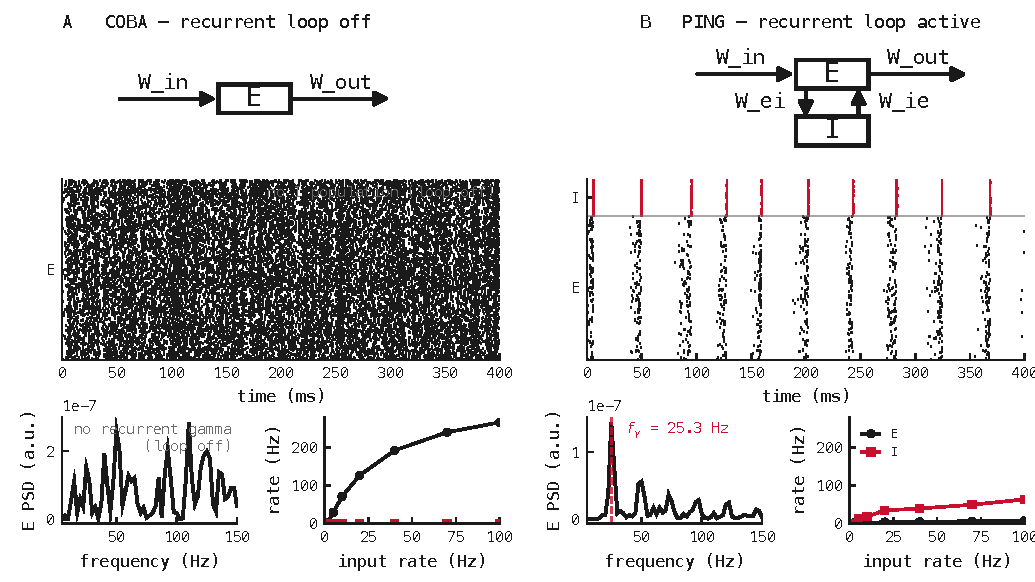
\includegraphics[width=\linewidth]{nb023_overview_compound.pdf}
  \caption{}\label{fig:1}
\end{figure}

\begin{figure}[!htbp]\centering   % nb057 — gamma onset / Hopf bifurcation
  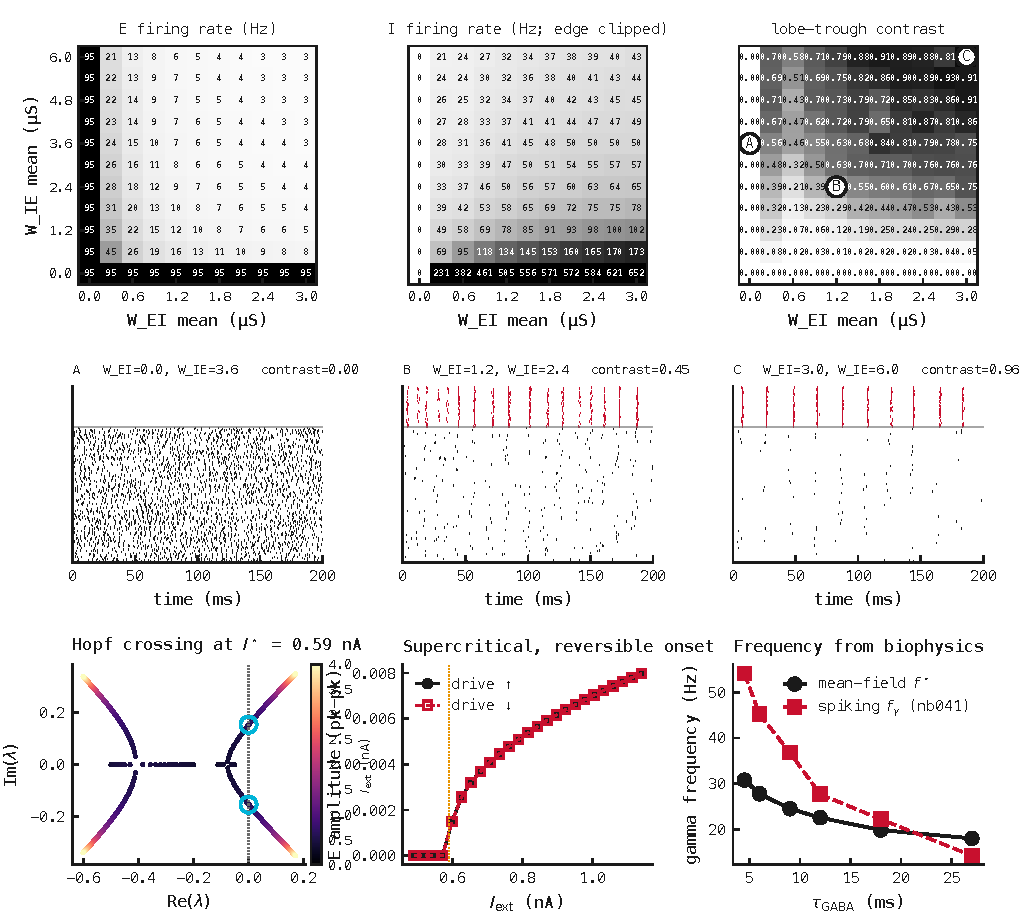
\includegraphics[width=\linewidth]{nb057_onset_super_compound.pdf}
  \caption{}\label{fig:2}
\end{figure}

\begin{figure}[!htbp]\centering   % nb025 — trained accuracy--rate frontier
  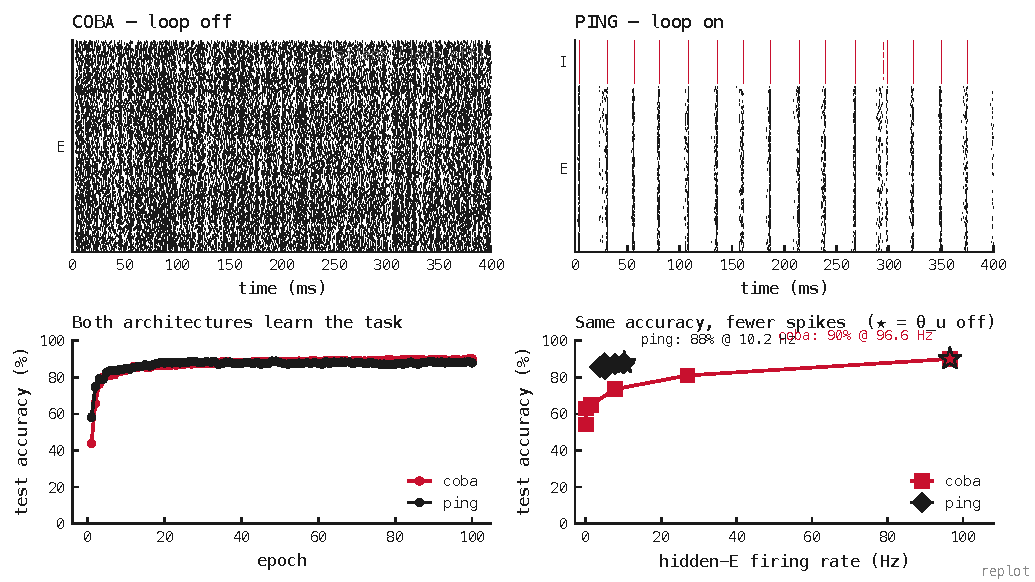
\includegraphics[width=\linewidth]{nb025_results_compound.pdf}
  \caption{}\label{fig:3}
\end{figure}

\begin{figure}[!htbp]\centering   % nb038 — loop transfer at inference
  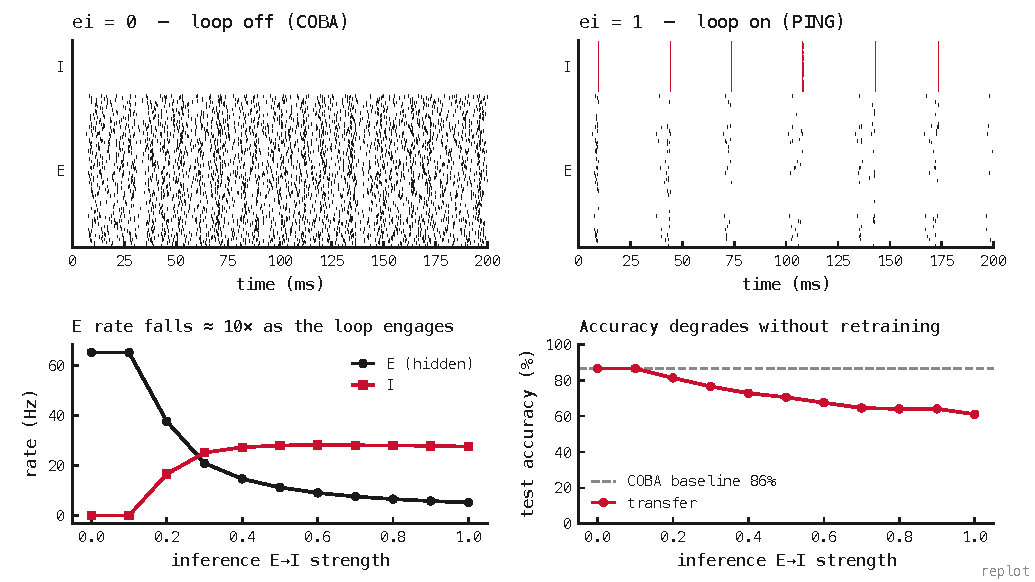
\includegraphics[width=\linewidth]{nb038_loop_transfer_compound.pdf}
  \caption{}\label{fig:4}
\end{figure}

\begin{figure}[!htbp]\centering   % nb049 — training prunes the loop
  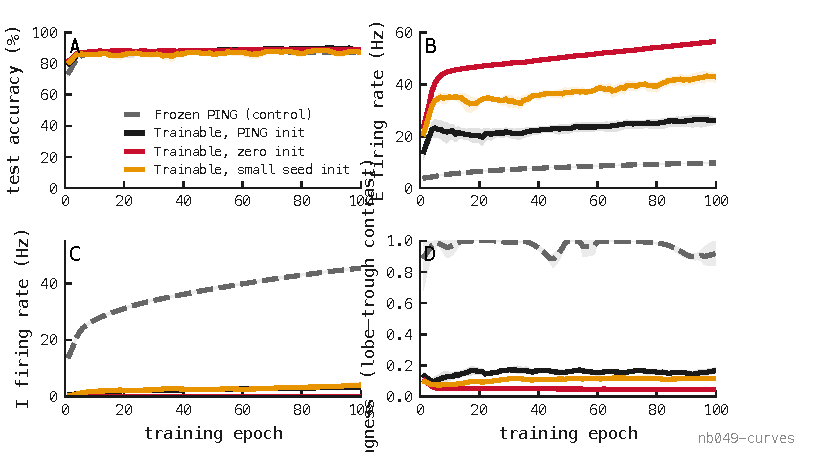
\includegraphics[width=\linewidth]{nb049_training_curves.pdf}
  \caption{}\label{fig:5}
\end{figure}

\begin{figure}[!htbp]\centering   % nb041 — rate law r_E = a + p f_gamma
  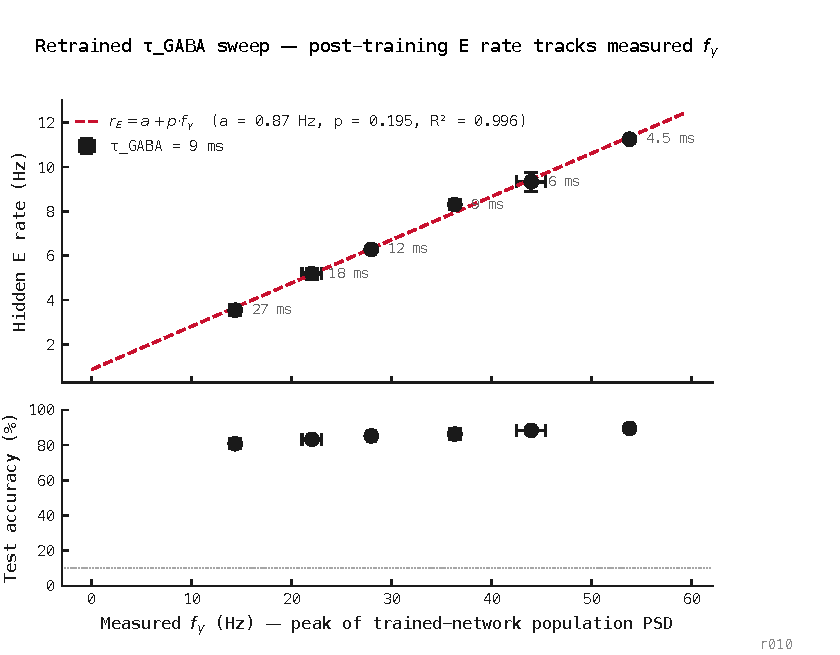
\includegraphics[width=\linewidth]{nb041_rate_vs_fgamma.pdf}
  \caption{}\label{fig:6}
\end{figure}

\begin{figure}[!htbp]\centering   % nb046 — spikes per cycle distribution
  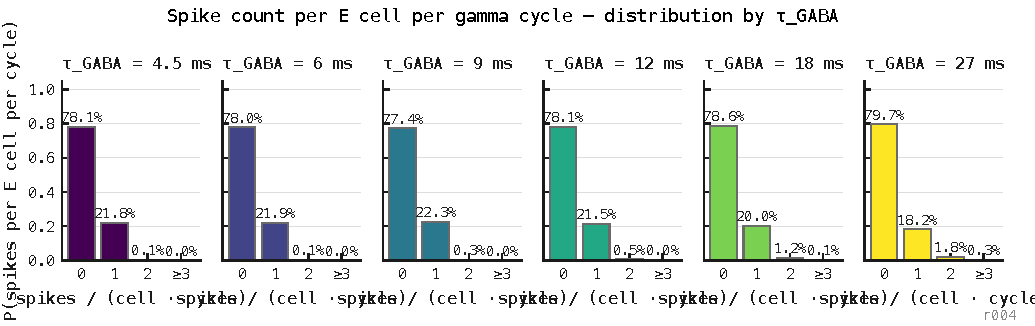
\includegraphics[width=\linewidth]{nb046_spikes_per_cycle_distribution.pdf}
  \caption{}\label{fig:7}
\end{figure}

\begin{figure}[!htbp]\centering   % nb047 — rate vs per-synapse W^IE
  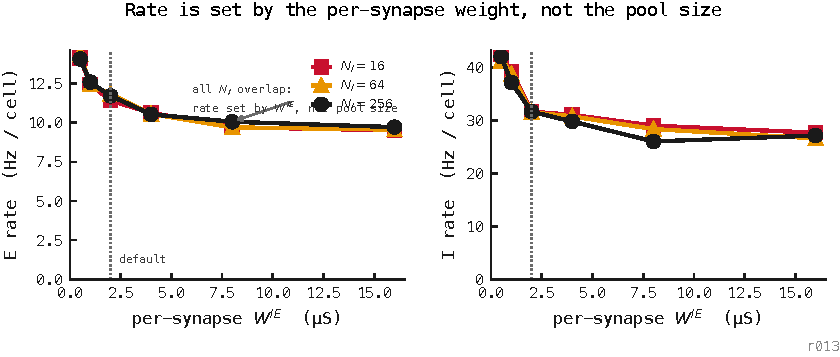
\includegraphics[width=\linewidth]{nb047_rate_vs_w_ie.pdf}
  \caption{}\label{fig:8}
\end{figure}

\begin{figure}[!htbp]\centering   % nb037 — drop/add perturbation asymmetry
  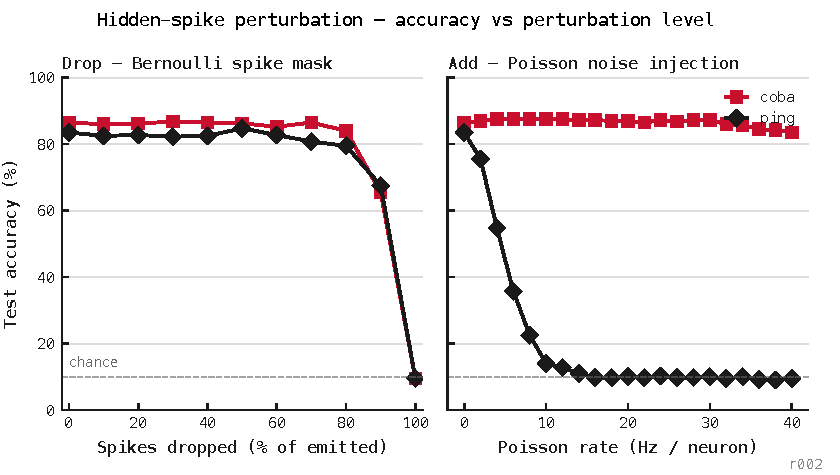
\includegraphics[width=\linewidth]{nb037_perturbation_curves.pdf}
  \caption{}\label{fig:9}
\end{figure}

\begin{figure}[!htbp]\centering   % nb042 — timing vs mean inhibition
  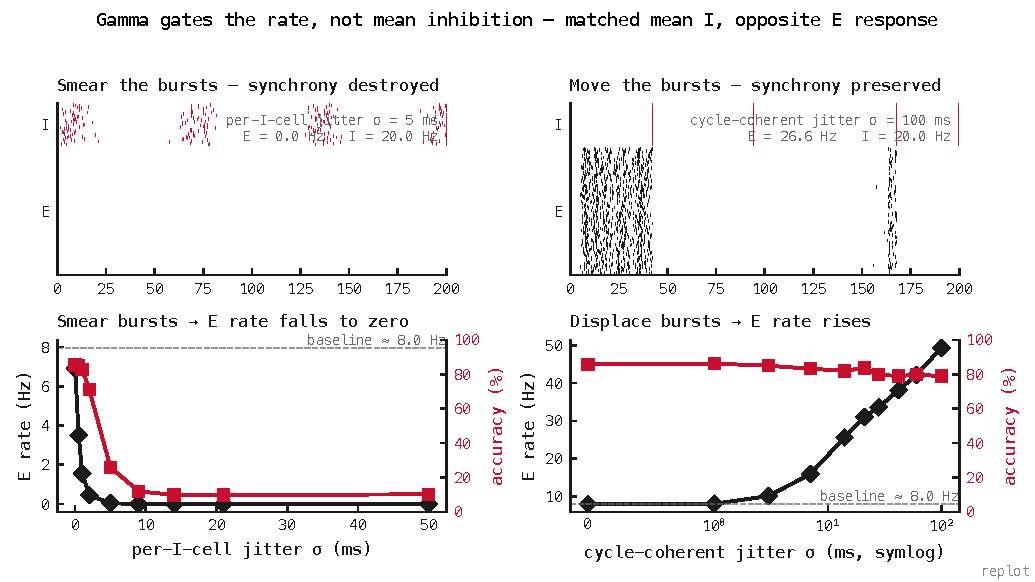
\includegraphics[width=\linewidth]{nb042_rhythm_compound.pdf}
  \caption{}\label{fig:10}
\end{figure}

\begin{figure}[!htbp]\centering   % nb044 — dt invariance
  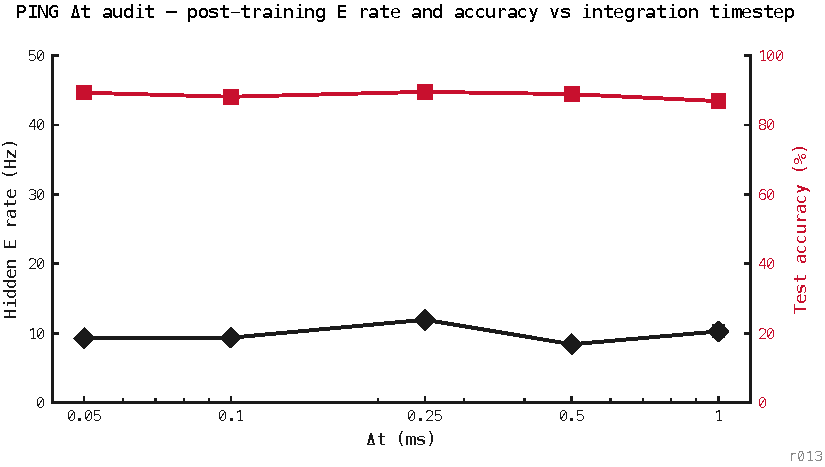
\includegraphics[width=\linewidth]{nb044_dt_sweep.pdf}
  \caption{}\label{fig:11}
\end{figure}

\begin{figure}[!htbp]\centering   % nb048 — streaming classification
  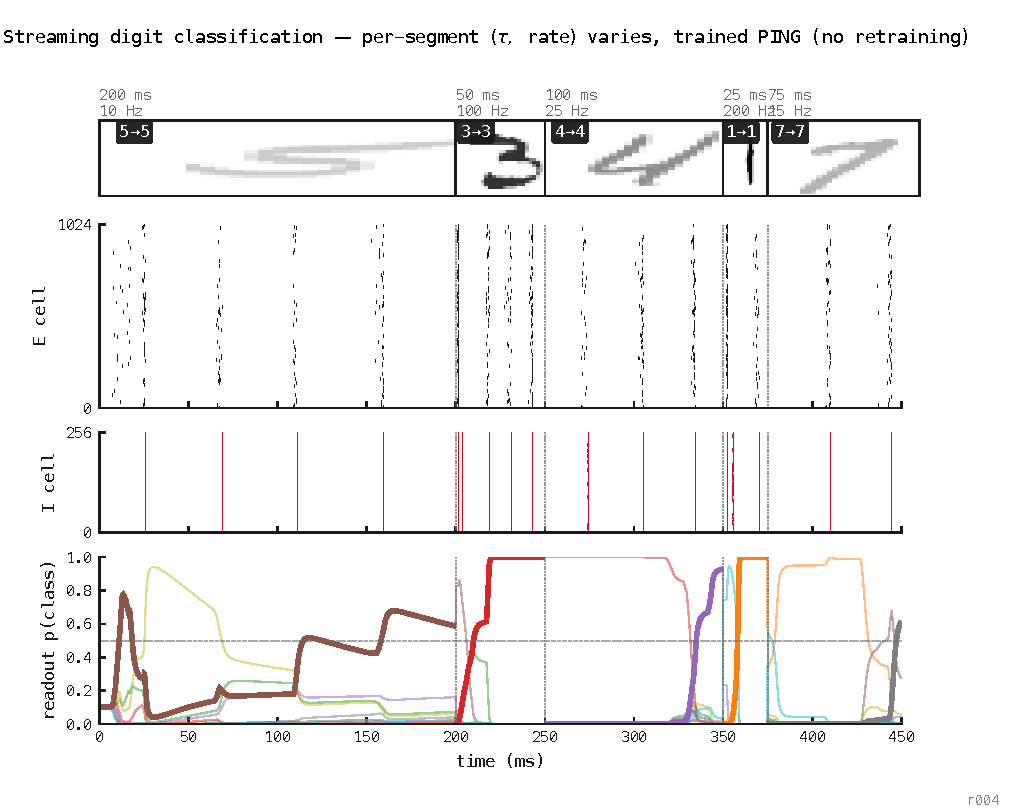
\includegraphics[width=\linewidth]{nb048_varying_headline_stream.pdf}
  \caption{}\label{fig:12}
\end{figure}

\begin{figure}[!htbp]\centering   % nb048 — accuracy grid (tau x rate)
  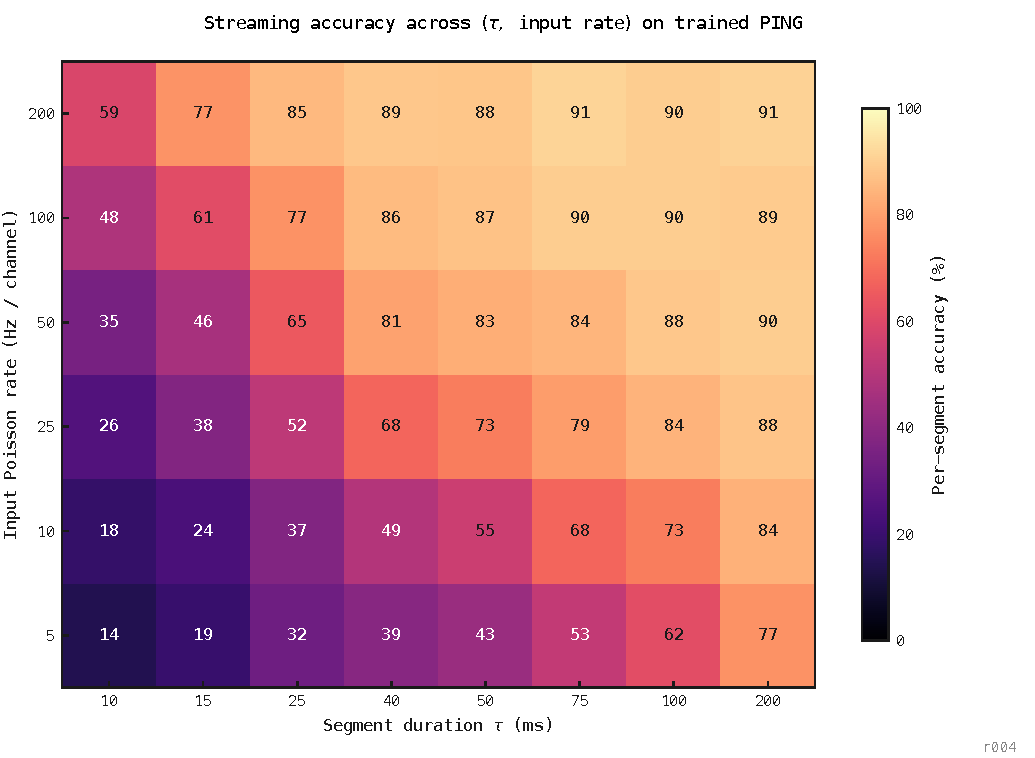
\includegraphics[width=\linewidth]{nb048_acc_grid_tau_rate.pdf}
  \caption{}\label{fig:13}
\end{figure}

\clearpage
\bibliographystyle{unsrtnat}
\bibliography{references}

\end{document}
